% Copyright (C)  2018  TANSORIER.
% Permission is granted to copy, distribute and/or modify this document
% under the terms of the GNU Free Documentation License, Version 1.3
% or any later version published by the Free Software Foundation;
% with no Invariant Sections, no Front-Cover Texts, and no Back-Cover Texts.
% A copy of the license is included in the section entitled "GNU
% Free Documentation License".

% https://www.gnu.org/licenses/fdl-1.3.html

% compress option to have horyzontal circle
\documentclass[compress,aspectratio=169]{beamer}

%%%%%%%%%%%%%%%%%%%%%%%%%%%%%%%%%%%%%%%%%%%%%%%%%%%%%%%%%%%%%%%%%%%%%

% Thèmes suppélmentaires
\useoutertheme[]{miniframes} % barre menu du haut
\setbeamertemplate{frametitle}[default] % replace le titre à la bonne place
\useinnertheme[shadow=true]{rounded} % arrondi les angles
\usecolortheme{orchid}
\usecolortheme{whale}

%\usepackage{xcolor}
%\definecolor{smileOrange}{RGB}{254,128,86}

\setbeamertemplate{footline}[text line]{
\textcolor{gray}{%
	\parbox{\linewidth}{\vspace*{-8pt}Smile\hfill\insertshortauthor\hfill\insertpagenumber/\inserttotalframenumber}}
}
\beamertemplatenavigationsymbolsempty

% Language
\usepackage[french]{babel}
\usepackage[utf8]{inputenc}
\usepackage[T1]{fontenc}
%\usepackage[latin1]{inputenc}

% Display Table Of Content spécific for smilebeamer
% Force to get empty
\AtBeginSection[]{}
\AtBeginSubsection[]{}
%{
%  \begin{frame}<beamer>
%  \frametitle{Plan}
%  \tableofcontents[currentsection]
%  \end{frame}
%}

% Change color of definiton block
\AtBeginEnvironment{definition}{%
	\setbeamercolor{block title}{use=example text,fg=example text.fg,bg=example text.fg!20!bg}
	\setbeamercolor{block body}{parent=normal text,use=block title,bg=block title.bg!50!bg}
}


% code coloration
\usepackage{listings}
% L'option "[fragile]" doit être rajouté au frame pour pouvoir utiliser correctement
% la police verbatim
\usepackage{color}
\lstset{
  breaklines=true,
  tabsize=4,
  backgroundcolor=\color[RGB]{49,54,59},
  basicstyle=\footnotesize\ttfamily\color{white},
  commentstyle=\itshape\color[RGB]{0,136,136},
  morecomment=[l]{\#},
  morekeywords={*,\$,\{,\}},
  stringstyle=\itshape\color[RGB]{218,116,0},
  showstringspaces=false,
  frame=LTBR,
}
\lstdefinestyle{shell}{
  language=bash,
  keywords={\$},
  keywordstyle=\bfseries\color[RGB]{66,198,66}
}
\lstdefinelanguage{diff}{
  morecomment=[f][\color{blue}]{@@},     % group identifier
  morecomment=[f][\color{red}]-,         % deleted lines 
  morecomment=[f][\color{green}]+,       % added lines
  morecomment=[f][\color{magenta}]{---}, % Diff header lines (must appear after +,-)
  morecomment=[f][\color{magenta}]{+++},
}

% Pour utiliser des colonnes
\usepackage{multicol}

% Pour integrer un pdf
\usepackage[final]{pdfpages}

% Pour les hyperliens
\usepackage{hyperref}

%%%%%%%%%%%%%%%%%%%%%%%%%%%%%%%%%%%%%%%%%%%%%%%%%%%%%%%%%%%%%%%%%%%%%
\title[U-Boot]{fitImage \& signature de paquets \\ \textbf{Introduction}}

\author[Mickaël Tansorier]{Mickaël Tansorier}

\date[Août 2018]{Présentation du fonctionnement des fitImage et \newline du fonctionnement de signature de paquets}
%%%%%%%%%%%%%%%%%%%%%%%%%%%%%%%%%%%%%%%%%%%%%%%%%%%%%%%%%%%%%%%%%%%%%

\begin{document}
%\tableofcontents[subsectionstyle=hide]

% *******************************
% ****     PAGE DE GARDE     ****
% *******************************

\begin{frame}
\titlepage
\end{frame}


% *******************************
% ****      INTRODUCTION     ****
% *******************************


\begin{frame}{Plan}
\tableofcontents[hideallsubsections]
\end{frame}

\section{Introduction}

\begin{frame}{Images Linux}
\begin{itemize}
	\item \textbf{Image}: image générique binaire
	\item \textbf{zImage}: image générique binaire compressé
	\item \textbf{uImage}: image avec une entête d'information utilisé par U-Boot
	\item \textbf{fitImage}: enveloppe d'image pouvant contenir plusieurs noyaux, devicetree, firmware. Chaque image peut être signé, et d'autres choses
\end{itemize}
\end{frame}

{
\setbeamercolor{background canvas}{bg=}
\includepdf[pages=12-13]{docs/Vasut--secure_and_flexible_boot_with_u-boot_bootloader.pdf}
}

{
\setbeamercolor{background canvas}{bg=}
\includepdf[pages=22]{docs/Josserand-schulz-secure-boot.pdf}
}

% *******************************
% ****     PRÉSENTATION      ****
% *******************************

\section{Construire fitImage}

\subsection{Les sources mainline}

\begin{frame}[fragile]
% Prevent first column disapear
\begin{columns}\begin{column}{0.2\textwidth}\end{column}\end{columns}
\begin{lstlisting}[style=shell,basicstyle=\tiny\ttfamily\color{white}]
KERNEL=/path/to/zImage
KEYNAME=my_key
\end{lstlisting}
\begin{columns}
\begin{column}{0.5\textwidth}
\begin{lstlisting}[style=shell,basicstyle=\tiny\ttfamily\color{white}]
/dts-v1/;

/ {
	description = "fitImage for sign Kernel image and DTB";
	#address-cells = <1>;

	images {
		kernel@1 {
			description = "Linux Kenel";
			data = /incbin/("%KERNEL%");
			type = "kernel";
			arch = "arm";
			os = "linux";
			compression = "none";
			load = <0x12000000>;
			entry = <0x12000000>;
			signature@1 {
				algo = "sha256,rsa4096";
				key-name-hint = "%KEYNAME%";
			};
		};
\end{lstlisting}
\end{column}
\begin{column}{0.5\textwidth}  
\begin{lstlisting}[style=shell,basicstyle=\tiny\ttfamily\color{white}]
		fdt@1 {
			description = "Devicetree";
			data = /incbin/("%DTB%");
			type = "flat_dt";
			arch = "arm";
			compression = "none";
			load = <0x18000000>;
			entry = <0x18000000>;
			signature@1 {
				algo = "sha256,rsa4096";
				key-name-hint = "%KEYNAME%";
			};
		};
	};
	configurations {
		default = "conf@1";
		conf@1 {
			kernel = "kernel@1";
			fdt = "fdt@1";
		};
	};
};
\end{lstlisting}
\end{column}
\end{columns}
\end{frame}

\begin{frame}[fragile]
Plusieurs type de signature sont disponible: \texttt{common/image-sig.c}
\begin{lstlisting}[style=shell,basicstyle=\tiny\ttfamily\color{white}]
struct image_sig_algo image_sig_algos[] = {
    {
        "sha1,rsa2048",
        rsa_sign,
        rsa_add_verify_data,
        rsa_verify,
        &checksum_algos[0],
    },
    {
        "sha256,rsa2048",
        rsa_sign,
        rsa_add_verify_data,
        rsa_verify,
        &checksum_algos[1],
    },
    {
        "sha256,rsa4096",
        rsa_sign,
        rsa_add_verify_data,
        rsa_verify,
        &checksum_algos[2],
    }

};
\end{lstlisting}
\end{frame}

\subsection{Ajouter les clés dans uboot}
\begin{frame}[fragile]
Crée un devicetree spécifique
\begin{lstlisting}
/dts-v1/;
/ {
	model = "Keys";
	compatible ="vendor,board";
	signature {
		key-%KEYNAME% {
			required = "image";
			algo = "sha256,rsa4096";
			key-name-hint = "%KEYNAME%";
		};
	};
};
\end{lstlisting}
\end{frame}

\begin{frame}[fragile]
Pour le générer le dtb
\begin{lstlisting}[style=shell]
dtc -p 4096 $(@D)/u-boot_pubkey.dts -O dtb -o $(@D)/u-boot_pubkey.dtb
\end{lstlisting}
Ce qui donne:
\begin{lstlisting}[style=shell]
$ cat u-boot_pubkey.dtb
vendor,board signature key-my_key image sha256,rsa4096 my_key modelcompatiblerequiredalgokey-name-hint
\end{lstlisting}
\end{frame}

\begin{frame}[fragile]
Pour y ajouter la clé public
\begin{lstlisting}[style=shell]
mkimage -D "-I dts -O dtb -p 4096" -f $(@D)/fitImage.its -K $(@D)/u-boot_pubkey.dtb -k $(@D) -r fitImage
\end{lstlisting}
Ce qui donne:
\begin{lstlisting}[style=shell]
$ cat u-boot_pubkey.dtb
vendor,board signature key-my_key
[...]
image sha256,rsa4096 my_key modelcompatiblerequiredalgokey-name-hintrsa,num-bitrsa,n0-inversersa,exponentrsa,modulusra,r-squaredsquared
\end{lstlisting}     
\end{frame}

\begin{frame}[fragile]
Pour s'assurer que le device tree contenant la clé public soit dans dans le binaire u-boot, il faut que cette option soit à non:
\begin{lstlisting}[style=shell]
BR2_TARGET_UBOOT_USE_CUSTOM_CONFIG
\end{lstlisting}
Pour ajouter dans notre U-boot alors que l'on a pas de dtb, on utiliser l'option EXT\_DTB de make:
\begin{lstlisting}[style=shell]
make CROSS_COMPILE=arm-linux-gnueabihf- EXT_DTB=u-boot_pubkey.dtb
\end{lstlisting}
\end{frame}


\subsection{Signer l'image noyau}
\begin{frame}[fragile]
Ok maintenant il faut siqner le kernel linux.\newline
Il faut le signer avant de compiler u-boot puisque pour ajouter la clé public au devicetree il faut executer mkimge avec en entrée l'its et en sortier le fitImage:
\begin{lstlisting}[style=shell]
mkimage -D "-I dts -O dtb -p 4096" -f $(@D)/fitImage.its -K $(@D)/u-boot_pubkey.dtb -k $(@D) -r fitImage
\end{lstlisting}
Le noyau Linux est bien construit avant U-boot, donc pas besoin d'ajouter de dépendance.
\end{frame}

% *******************************
% ****     PRÉSENTATION      ****
% *******************************
\section{Paramétrer buildroot - fitImage}

\subsection{uboot}
\begin{frame}[fragile]
J'ai rajouté quelques config dans buildroot.
\begin{lstlisting}[style=shell]
BR2_PACKAGE_UBOOT_TOOLS_FIT_SUPPORT=y
BR2_PACKAGE_UBOOT_TOOLS_FIT_SIGNATURE_SUPPORT=y
BR2_PACKAGE_HOST_UBOOT_TOOLS=y
BR2_PACKAGE_HOST_UBOOT_TOOLS_FIT_SUPPORT=y
BR2_PACKAGE_HOST_UBOOT_TOOLS_FIT_SIGNATURE_SUPPORT=y

BR2_TARGET_UBOOT_NEEDS_OPENSSL=y

BR2_TARGET_UBOOT_SIGN_FITIMAGE=y
BR2_TARGET_UBOOT_ITS="$(CONFIG_DIR)/board/eolane/modx6/fitImage.its"
BR2_TARGET_UBOOT_SIGN_DTS="$(CONFIG_DIR)/board/eolane/modx6/u-boot_pubkey.dts"
BR2_TARGET_UBOOT_KEY_NAME="my_key"
BR2_TARGET_UBOOT_KEY_SERVER="bep@hgweb:/home/apache/distribution/keys/"
\end{lstlisting}
\end{frame}

\begin{frame}[fragile]{Vérification de la signature}
il est possible de tester la signature d'une image avec:
\begin{lstlisting}[style=shell]
fit_check_sign -f output/images/fitImage -k u-boot_pubkey.dtb
\end{lstlisting}
dans \texttt{./output/build/host-uboot-tools-2017.07/tools/fit\_check\_sign}
\end{frame}

\begin{frame}[fragile]
Documentation:
\begin{itemize}
\item \url{https://elinux.org/images/e/e0/Josserand-schulz-secure-boot.pdf}
\item \url{https://www.denx.de/wiki/pub/U-Boot/Documentation/multi_image_booting_scenarios.pdf}
\item \url{https://elinux.org/images/8/8a/Vasut--secure_and_flexible_boot_with_u-boot_bootloader.pdf}
\end{itemize}
\end{frame}

% *******************************
% ****     PRÉSENTATION      ****
% *******************************
\section{Signature de paquets}

\subsection{Générer les clés}
\begin{frame}[fragile]
Il faut une clé paire de clé:
\begin{lstlisting}[style=shell]
$ openssl genrsa -out my_key.key 4096
$ openssl req -batch -new -x509 -key my_key.key -out my_key.crt
\end{lstlisting}
Pour extraire le clé publique du certificat
\begin{lstlisting}[style=shell]
openssl x509 -pubkey -noout -in my_key.crt > my_key.pub
\end{lstlisting}
\end{frame}

\subsection{Signer}
\begin{frame}[fragile]
Pour signer:
\begin{lstlisting}[style=shell]
openssl dgst -sha256 -sign my_key.key -out file_to_sign.sha256 file_to_sign
\end{lstlisting}
Si la signature est sous forme binaire, on peut la convertir sous forme textuel:
\begin{lstlisting}[style=shell]
openssl base64 -in file_to_sign.sha256 -out file_to_sign.sign
\end{lstlisting}
\end{frame}

\subsection{Vérifier}
\begin{frame}[fragile]
Pour signer:
\begin{lstlisting}[style=shell]
openssl dgst -sha256 -verify my_key.pub -signature file_to_sign.sha256 file_to_sign
\end{lstlisting}
Si la signature est sous forme binaire, on peut la convertir sous forme textuel:
\begin{lstlisting}[style=shell]
openssl base64 -d -in file_to_sign.sign -out file_to_sign.sha256
\end{lstlisting}
\end{frame}


% *******************************
% ****     PRÉSENTATION      ****
% *******************************
\section*{Conclusion}
\begin{frame}
\begin{center}
\begin{huge}
Question ?
\end{huge}
\end{center}
\begin{center}
\textcolor{gray}{\tiny{Enfin je vais essayer de répondre...}}
\end{center}
\end{frame}

\end{document}
